\documentclass{article}
\usepackage[utf8]{inputenc}

\title{Analysis_1b_V1.0}
\author{thi.schwaller444 }
\date{December 2019}
\usepackage{multicol}
\usepackage{mathtools}
\usepackage{pdfpages}
\usepackage[a4paper,width=150mm,top=25mm,bottom=25mm]{geometry}
\pagestyle{myheadings}
\markright{Thierry Schwaller / https://github.com/tschwall/Zusammenfassungen}
\begin{document}
\section{Kurvendiskussion S.261}
\textbf{1. Definitionsbereich bestimmen} \\
\textbf{2. Nullstellen bestimmen} \\
\textbf{3. Symmetrie untersuchen (f(-x) = f(x)) / Periodizität} \\
\textbf{4. Verhalten in die Unendlichkeit}
\begin{equation*}
    \lim\limits_{n \rightarrow \pm \infty}{f(x)}
\end{equation*}
\textbf{5. Extremalwerte / Wendepunkte} \\
Erste Ableitung = 0 setzen.\\
Wenn \textbf{zweite Ableitung $>$ 0} ist ist der gefundene Punkt ein \textbf{Minimum} wenn die \textbf{zweite Ableitung $<$ 0} ist ist der Punkt ein \textbf{Maximum}. \\
Wenn die \textbf{zweite Ableitung = 0} ist und die \textbf{dritte Ableitung $\neq$ 0}, dann liegt ein \textbf{Wendepunkt} vor. \\ \\
\textbf{6. Krümmungsverhalten} \\
Wenn f''(x) $<$ 0 dann \textbf{konkav, rechtsgekrümmt, Tangente über der Funktion} \\
Wenn f''(x) $>$ 0 dann \textbf{konvex, linksgekrümmt, Tangente unter der Funktion} \\ \\
\textbf{7. Grenzwertverhalten}\\
An Randstellen, bei Definitionslücken und evtl. Asymptotik
\section{Taylor-Polynome s.455}
Taylor-Polynome von f(x): \\
\textbf{1. Bestimmen der ersten n Ableitungen von f(x)} \\
\textbf{2. Werte an Arbeitsstelle a berechnen} \\
\textbf{3. Als Summe notieren} \\
\begin{equation*}
    f(x) = \sum_{k=0}^n \frac{f^{(k)}(a) * (x - a)^k)}{k!}
\end{equation*}
\textbf{$p_n(x)$ beinhaltet die $f^{(n)}$ te Ableitung}
\sub section{Lagrange}
\begin{multicols}{2}
\begin{equation*}
    R_n = | \frac{f^{n+1}(\xi)}{(n + 1)!}h^{n+1} |
\end{equation*}
\columnbreak
\begin{center}
    n $\rightarrow$ Höchste Ableitung in  Taylor \\
h $\rightarrow$ Abstand zur Arbeitsstelle \\
$\xi \rightarrow$ Zahl im Bereich von $x_{max}$ und $x_{min}$
\end{center}
\end{multicols}
\section{Trigonometrie}
\textbf{Limits:} \\
\textbf{Arctangents} $\rightarrow +\infty = \frac{\pi}{2}$ $\rightarrow -\infty = - \frac{\pi}{2}$ \\
\textbf{Arccotangents} $\rightarrow +\infty = 0$ $\rightarrow -\infty = {\pi}$ 
\newpage
\section{Fehlerfortplanzung}
Relative Fehler:
\begin{equation*}
    \frac{dy}{y} = \frac{f'(x) * dx}{f(x)} 
\end{equation*}
Absolute Fehler:
\begin{equation*}
    dy = f'(x)*dx
\end{equation*}
\section{Integrierbare Funktionen}
\begin{center}
    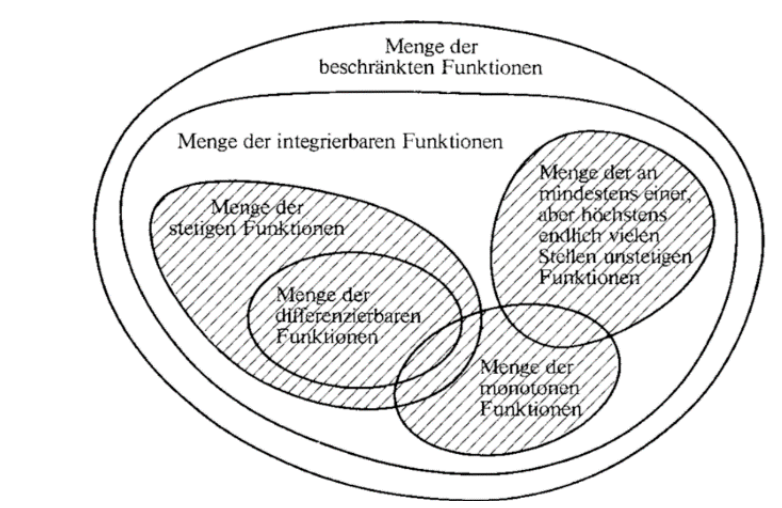
\includegraphics[width=0.35\textwidth]{MengenIntegral.PNG}
\end{center}
\section{Winkel zwischen Funktionen}
\begin{multicols}{2}
\begin{center}
    Allgemein:
\begin{equation*}
    tan(\alpha) =\frac{m_1 - m_2}{1 + m_1 * m_2}
\end{equation*}
\end{center}
\columnbreak
\begin{center}
    Senkrecht:
\begin{equation*}
    m1 = -\frac{1}{m_2}
\end{equation*}
\end{center}
\end{multicols}
\section{Mittelwertsatz}
\begin{multicols}{2}
\textbf{Differenzrechnungen:}
\begin{center}
    \begin{equation*}
    \frac{f(b) - f(a)}{b-a} = f'(\xi)
    \end{equation*}
\end{center}
\columnbreak
\textbf{MWS Integralrechnen:}
\begin{center}
    \begin{equation*}
    \int_{a}^{b}f(x)dx = (b - a)f(\xi) 
    \end{equation*}
\end{center}
\end{multicols}
\section{Integralfunktionen / Stammfunktionen}
An Beispiel von $f(t)= cos(t)$: \\
\textbf{Stammfunktion:} 
\begin{equation}
    sin(t) + K
\end{equation}
\textbf{Integralfunktion (Schneidet immer die X - Achse):}
\begin{equation*}
    I(x) = \int_{c}^{x}cos(t)dt = sin(t)|_{c}^{x} = sin(x) - sin(c)
\end{equation*}
\section{Wichtige Seiten Bronstein}
\textbf{n-te Ableitung} $\rightarrow$ S.452 
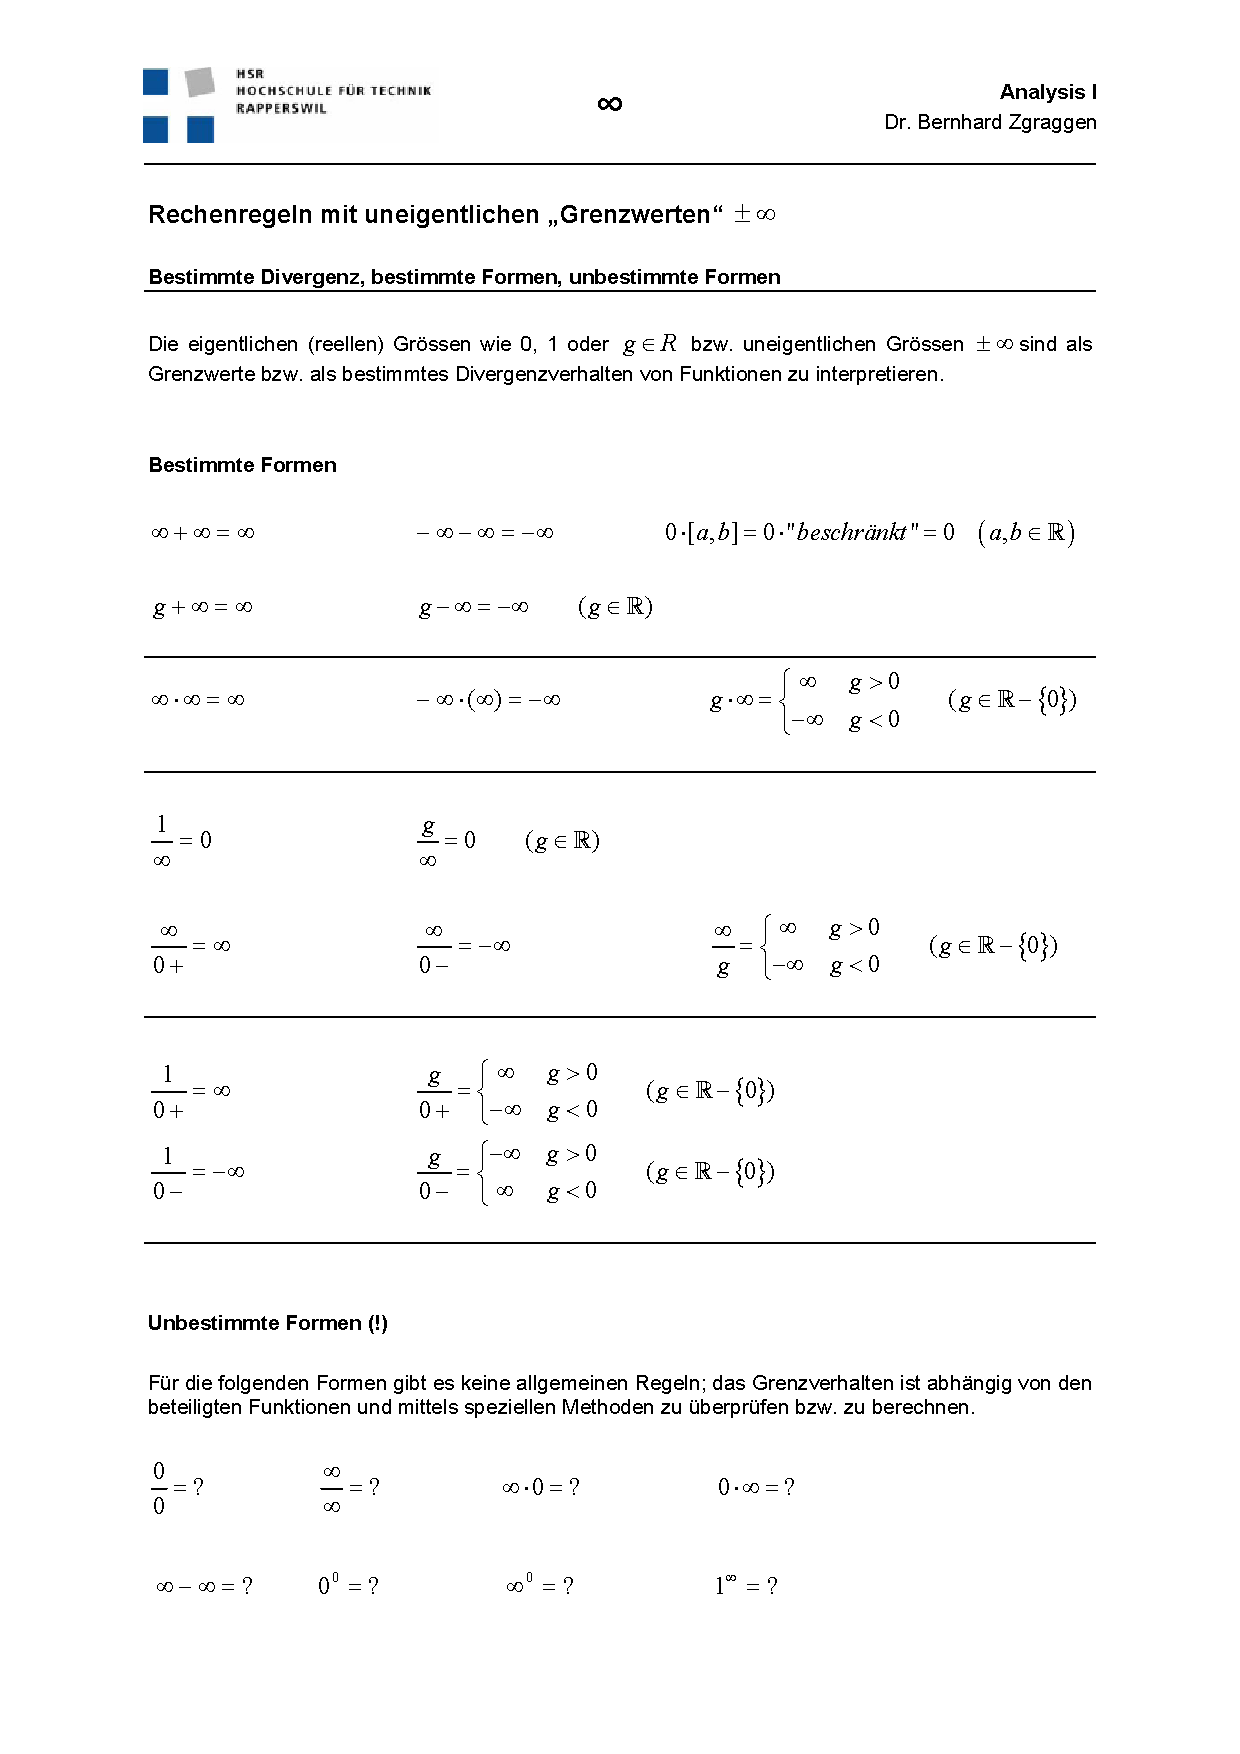
\includepdf[pages=1, scale=1, frame = false]{An1UnterlagenInfinity}
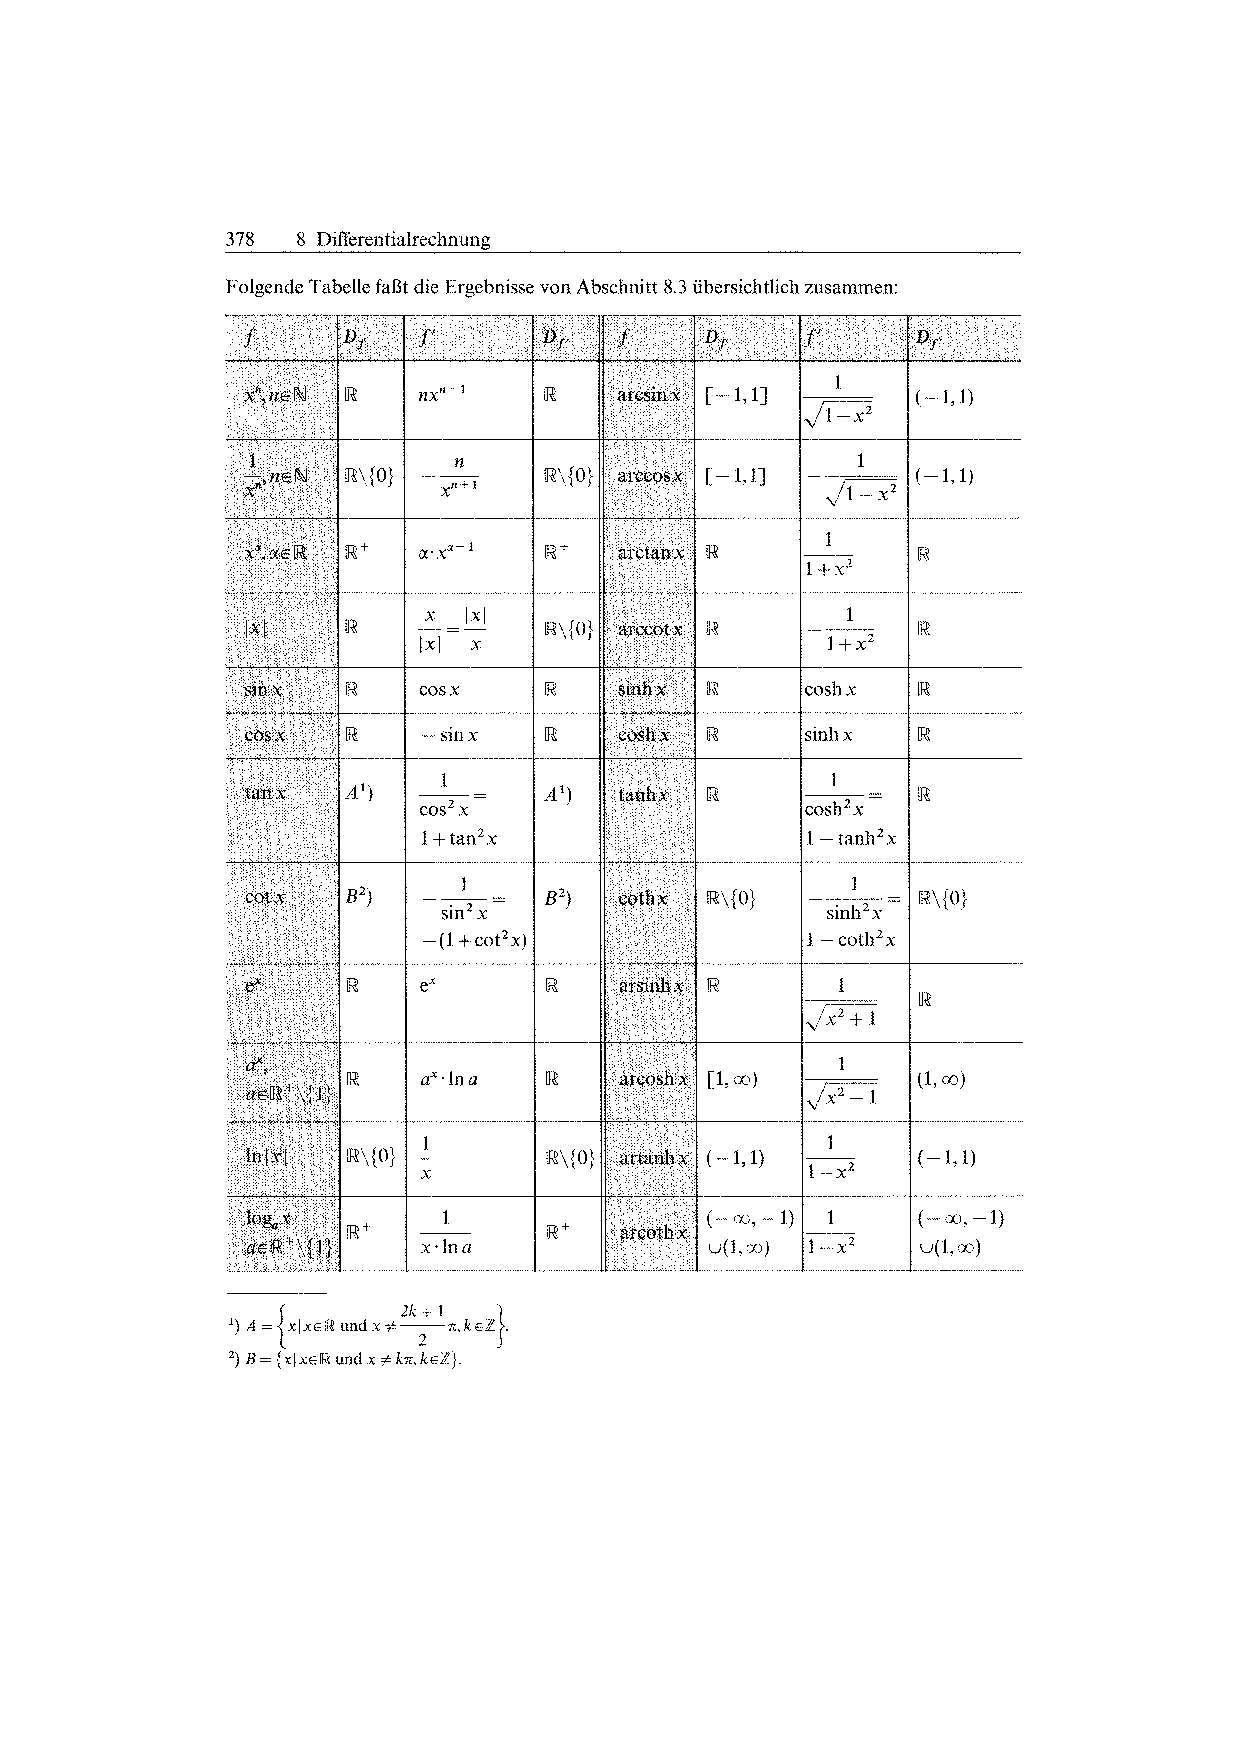
\includepdf[pages=1, scale=1, frame = false]{Ableitung}
\end{document}